\documentclass[ngerman]{article}

\usepackage[margin=2.75cm]{geometry}
\usepackage[T1]{fontenc}
\usepackage[utf8]{inputenc}
\usepackage{textcomp}
\usepackage{graphicx}
\usepackage{babel}
\usepackage{titlesec}
\usepackage{xcolor}

\begin{document}

\section*{Einleitung}
Die Informationsgesellschaft unserer Tage ist ohne Computer und Datennetze nicht mehr denkbar.
In\-for\-ma\-tions- und Kommunikationstechnologien spielen eine wichtige Rolle für den Zugang zu Bildung, Kultur und Wissenschaft.
Trotz immer neuer und schnellerer digitaler Kommunikationsformen ist der Zugang zu diesen Technologien nicht allen Menschen gleichermaßen möglich.
Der Verein zur Förderung freier Netze Hessen hat sich zur Aufgabe gemacht, den öffentlichen, gleichberechtigten und nicht diskriminierenden Zugangs zu Informationen, unabhängig von kommerziellen Interessen zu fördern.
Dies wird erreicht durch den Aufbau und Betrieb einer entsprechenden Infrastruktur, sowie die Aufklärung der breiten Masse im Bezug auf die Auswirkungen freie zugänglicher Netze auf die Gesellschaft.

\section*{Was sind freie Netze}

\section*{Wie lassen sich solche Netze realisieren}
Hinleitung zu Freifunk.

\section*{Was ist Freifunk}
Bei Freifunk handelt es sich um ein Projekt zum Aufbau einer unabhängigen Netzinfrastruktur unter Nutzung der WLAN-Technik.

Dafür werden verwendet Standard-WLAN-Router verwendet, die aus dem privaten Hausgebrauch bekannt sein dürften. 
Auf einen solchen WLAN-Router wird eine speziellen Firmware (das Betriebssystem des WLAN-Routers) installiert, mittels der die Vernetzung von Freifunk-Geräten untereinander ermöglicht wird.
Die Freifunk-Firmware wird als Open Source Projekt dezentral in den regionalen Freifunk Verbänden entwickelt und interessierten zur freien Nutzung zur Verfügung gestellt.
Änderungen und Erweiterungen, die in einem regionalen Verband durchgeführt werden, stehen anschließend wiederum allen Verbänden zur freien Nutzung zur Verfügung.
   
Ein mit der Freifunk-Firmware ausgestatteter WLAN-Router ist in der Lage, weitere Freifunk-Geräte in seiner Nähe automatisch zu erkennen und sich mit diesen per WLAN zu verbinden. 
Es entsteht ein sogenanntes Mesh-Netzwerk, das sich dadurch auszeichnet, dass ein Knoten mit einer Vielzahl anderer Knoten verbunden ist.
Durch ein intelligentes Routing-Protokolls, das speziell für unzuverlässige Funknetze entworfen wurde, ist die Wegfindung innerhalb des Netzes und somit die Kommunikation untereinander möglich.

Die Abbildung zeigt, wie durch den Betrieb von Freifunk-Knoten in den Wohnungen von Bürgern ein miteinander verbundenes Netzwerk entsteht, das unabhängig von kommerziellen Anbietern funktioniert.
Nutzer, die sich mit dem Freifunk-Netz verbinden, können untereinander kommunizieren und Daten austauschen, ohne dass dazu ein Internetanschluss benötigt wird.

\begin{figure}[h!]
	\centering
	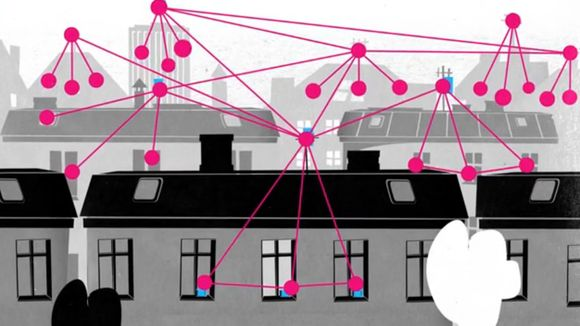
\includegraphics[width=.7\textwidth]{freifunk-mesh}
	%\caption{}
	\label{fig:freifunkwolke}
\end{figure}

\section*{Wie wird das vom Förderverein Freie Netze Hessen umgesetzt}
  \begin{itemize}
    \item Handelsübliche WLAN Router
    \item Software des Routers mit der sich die Vernetzung realisieren lässt
    \item Software ist unter einer freien Lizenz und quelloffen
    \item Plattform für die Mitarbeit und Unterstützung zur Weiterentwicklung der Freifunk Software
    \item Aufklärung wie funktionieren Computernetze und wie ist das bei Freifunk konkret umgesetzt
    \item wie kann diese Technologie sicher genutzt werden
    \item Förderung gemeinschaftlicher Arbeit, Treffpunkt für Leute die an diesem Thema mitarbeiten wollen.
  \end{itemize}

\end{document}